% USEFUL LINKS:
% -------------
%
% - UiO LaTeX guides:          https://www.mn.uio.no/ifi/tjenester/it/hjelp/latex/
% - Mathematics:               https://en.wikibooks.org/wiki/LaTeX/Mathematics
% - Physics:                   https://ctan.uib.no/macros/latex/contrib/physics/physics.pdf
% - Basics of Tikz:            https://en.wikibooks.org/wiki/LaTeX/PGF/Tikz
% - All the colors!            https://en.wikibooks.org/wiki/LaTeX/Colors
% - How to make tables:        https://en.wikibooks.org/wiki/LaTeX/Tables
% - Code listing styles:       https://en.wikibooks.org/wiki/LaTeX/Source_Code_Listings
% - \includegraphics           https://en.wikibooks.org/wiki/LaTeX/Importing_Graphics
% - Learn more about figures:  https://en.wikibooks.org/wiki/LaTeX/Floats,_Figures_and_Captions
% - Automagic bibliography:    https://en.wikibooks.org/wiki/LaTeX/Bibliography_Management  (this one is kinda difficult the first time)
%
%                              (This document is of class "revtex4-1", the REVTeX Guide explains how the class works)
%   REVTeX Guide:              http://www.physics.csbsju.edu/370/papers/Journal_Style_Manuals/auguide4-1.pdf
%
%
% COMPILING THE .pdf FILE IN THE LINUX TERMINAL
% ---------------------------------------------
%
% [terminal]$ pdflatex report_example.tex
%
% Run the command twice, always.
%
% When using references, footnotes, etc. you should run the following chain of commands:
%
% [terminal]$ pdflatex report_example.tex
% [terminal]$ bibtex report_example
% [terminal]$ pdflatex report_example.tex
% [terminal]$ pdflatex report_example.tex
%
% This series of commands can of course be gathered into a single-line command:
% [terminal]$ pdflatex report_example.tex && bibtex report_example.aux && pdflatex report_example.tex && pdflatex report_example.tex
%
% ----------------------------------------------------



% \documentclass[english,notitlepage,reprint,nofootinbib]{revtex4-2}  % defines the basic parameters of the document
\documentclass[english,notitlepage,reprint,nofootinbib]{revtex4-2}  % defines the basic parameters of the document
% If you want a single-column, remove "reprint"

% Allows special characters (including æøå)
\usepackage[utf8]{inputenc}
% \usepackage[english]{babel}

% Note that you may need to download some of these packages manually, it depends on your setup.
% It may be usefult to download TeXMaker, because it includes a large library of the most common packages.

\usepackage{physics,amssymb}  % mathematical symbols (physics imports amsmath)
\include{amsmath}
\usepackage{graphicx}         % include graphics such as plots
\usepackage{xcolor}           % set colors
\usepackage{hyperref}         % automagic cross-referencing
\usepackage{listings}         % display code
\usepackage{subfigure}        % imports a lot of cool and useful figure commands
% \usepackage{float}
%\usepackage[section]{placeins}
\usepackage{algorithm}
\usepackage[noend]{algpseudocode}
\usepackage{subfigure}
\usepackage{tikz}
\usetikzlibrary{quantikz}
% defines the color of hyperref objects
% Blending two colors:  blue!80!black  =  80% blue and 20% black
\hypersetup{ % this is just my personal choice, feel free to change things
    colorlinks,
    linkcolor={red!50!black},
    citecolor={blue!50!black},
    urlcolor={blue!80!black}}


% ===========================================


\begin{document}

\title{FYS4150 - Project 1\\[0.5em]
  \small \href{https://github.com/isakrukan/FYS4150/tree/main/Project1}{\texttt{github.com/isakrukan/FYS4150/Project1}}
}
\author{Isak Cecil Onsager Rukan} % self-explanatory
\date{\today}                             % self-explanatory
\noaffiliation                            % ignore this, but keep it.
\maketitle
The one-dimensional Poisson can be written as 
\begin{align}
    -\frac{d^2u}{dx^2} = f(x),  \label{eq:Poisson}
\end{align}
where $f(x)$ is some known function. In this project we let \(x\in[0,1]\) and
\begin{align}
    f(x) = 100e^{-10x}, \label{eq:f_x}
\end{align}
together with the following boundary conditions
\begin{align}
    u(0)=0, \quad u(1)=0. \label{eq:boundary_condition}
\end{align}
\section{Problem 1}
Let $v(x)=d/dx u(x)$. Integrating \eqref{eq:Poisson} leads to 
\begin{align}
    -v(x) &= 100\int dxe^{-10x}
    \notag \\
    &= -10e^{-10x} + C,
\end{align}
which means that 
\begin{align}
    u(x) &= \int v(x) 
    \notag \\
    &= -e^{-10x} - Cx + D.
\end{align}
Here $C$ and $D$ are some constants which are determined by the boundary conditions in \eqref{eq:boundary_condition}. Concretely, \(u(0)=0\) leads to $D=1$ and then \(u(1)=0\) sets \(C=-(1-e^{-10})\). Hence,
\begin{align}
    u(x) = 1 - (1 - e^{-10x})x - e^{-10x}.  \label{eq:u_x}
\end{align}
\section{Problem 2}
Using \href{https://github.com/isakrukan/FYS4150/blob/main/Project1/Code/problem2.cpp}{problem2.cpp} we compute $u(x)$ numerically for $N=10^4$ points. The result is written to \href{https://github.com/isakrukan/FYS4150/blob/main/Project1/Code/problem2.txt}{problem2.txt} and Fig. \ref{fig:u_x} is made in \href{https://github.com/isakrukan/FYS4150/blob/main/Project1/Code/problem2.py}{problem2.py}.
\begin{figure}[h!]
    \centering
    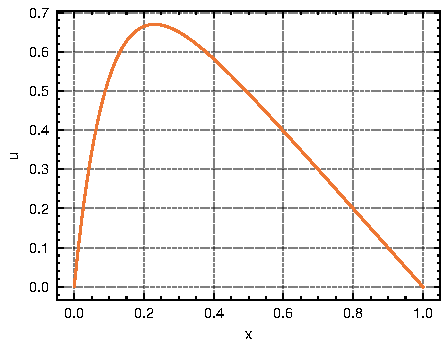
\includegraphics{Figs/problem2.pdf}
    \caption{Eq. \eqref{eq:u_x} using $N=10^4$ points.}
    \label{fig:u_x}
\end{figure}

\section{Problem 3}
The second derivative of $u(x)$, appearing on the R.H. side of \eqref{eq:Poisson} may be written as
\begin{align}
    \frac{d^2}{dx^2}u(x) = \lim_{h\rightarrow 0} \frac{u(x+h) -2u(x) + u(x-h)}{h^2}.    \label{eq:second_order_derivative}
\end{align}
To approximate this limit numerically, let $h$ be small and $\vec{x}$ be an array of $n$ points equispaced from zero to one. Eq. \eqref{eq:second_order_derivative} can then be approximated up to order $\mathcal{O}(h^2)$:
\begin{align}
    \frac{d^2}{dx^2}u(x)\vert_{x_i} = \frac{u(x_{i+1}) - 2u(x_i) + u(x_{i-1})}{h^2} + \mathcal{O}(h^2).  \label{eq:discretized_version_second_derivative}
\end{align}   
Since, according to \eqref{eq:Poisson}, the second derivative of $u(x)$ equals $-f(x)$, we can write \eqref{eq:discretized_version_second_derivative} as  
\begin{align}
    -h^2f(x_i) = \frac{u(x_{i+1}) - 2u(x_i) + u(x_{i-1})}{h^2} + \mathcal{O}(h^2). \label{eq:Poisson_disc}
\end{align}

\section{Problem 4}
Let $\vec{v} = (v_1,...,v_{n})$ be a vector whose $i$-th component is thought of as representing the numerical implementation (so ignoring the order $\mathcal{O}(h^2)$) of $u_{i+1}$.
Eq. \eqref{eq:Poisson_disc} can then be written as 
\begin{align}
    -v_{i-1} + 2v_{i} - v_{i+1} = h^2f(x_i).    \label{eq:numerical_v}
\end{align}
Further, 
let $\vec{g}$ be the vector of length \(n\), given by componentwise as 
\begin{align}
    \vec{g}_{i} = h^2f(x_{i+1}), i = 2, ..., n-1, 
\end{align}
and \(\vec{g}_{1} = h^2f(x_{1}) + u(0)\), \(\vec{g}_{n} = h^2f(x_{n}) + u(1)\). Then, if we let $A$ be the \(n\times n\)-matrix given by
\begin{align}
    A = \begin{pmatrix}
        2 & -1 & 0 & \cdots & 0 \\
        -1 & 2 & -1 & \ddots & \vdots \\
        0 & -1 & 2 & \ddots & 0 \\
        \vdots & \ddots & \ddots & \ddots & -1 \\
        0 & \cdots & 0 & -1 & 2
    \end{pmatrix},
\end{align}
we can represent \eqref{eq:numerical_v} as 
\begin{align}
    A\vec{v} = \vec{g}. \label{eq:as_matrix_multiplication}
\end{align}
To see that this explicitly, multiply the matrix $A$ with $\vec{v}$, which gives $A\vec{v}$ componentwise as
\begin{align}
    (A\vec{v})_{i} &= -v_{i-1} + 2v_{i} - v_{i+1}, \quad i = 2, ..., n-1.
\end{align}
For \(i=0\): \((A\vec{v})_{0} = 2v_{0} - v_{1}\), and \(i=n\): \((A\vec{v})_{n} = -v{n-1} + 2v_{n}\).



\section{Problem 5}
The vector $\vec{v}$ does not contain the boundary points corresponding to $x_{0}=0$ and $x_{N-1}=1$. Let the vector $\vec{v}^*$ be given by 
\begin{align}
    \vec{v}^* = (u(0), \vec{v}, u(1)).
\end{align}
Then, clearly, \(\vec{v}^*\) is a vector of length $n$ and when solving \eqref{eq:as_matrix_multiplication} we will obtain $\vec{v}$, which is \(\vec{v}^*\) excluding its first and last component.

\section{Problem 6} \label{sec:problem6}
Consider now $A$ as a general tridiagonal matrix with vectors $\vec{a}, \ \vec{b}$ and \(\vec{c}\) representing the subdiagonal, main diagonal and superdiagonal, respectively. When solving \eqref{eq:as_matrix_multiplication} we may then use a number of row operations on $A$, such that it turns into a matrix $\tilde{A}$ with all entries below the diagonal equal to zero. These row operations naturally alters the $\vec{\tilde{g}}$ on R.H. side of \eqref{eq:as_matrix_multiplication} into a vector $\tilde{g}$, at which point the solution to \eqref{eq:as_matrix_multiplication} can then be simply read of by multiplying out $\tilde{A}\vec{v} = \vec{\tilde{g}}$.

Let $R_{i}$ denote the $i$-th row of \eqref{eq:as_matrix_multiplication}. In the following, when writing $\overset{aR_i-b R_j}{\rightarrow}$, we mean the row operation of subtracting $b$ times row \(j\) from \(a\) times row \(i\). When applying a row operation to the $i$-th row, we write \(\tilde{b}_{j}\) and \(\tilde{g}_j\) as the resulting new \(j\)-th component of the vector \(\vec{b}\) and \(\vec{g}\), respectively. We have:
\begin{widetext}
\begin{align}
    &\left[\begin{array}{cccccc|c}
        R_1: & b_1 & c_1 & 0 & \cdots & 0  & g_1\\
        R_2: & a_{2} & b_2 & c_2 & \ddots & \vdots  & g_2\\
        R_3: & 0 & a_{3} & b_3 & \ddots & 0  & g_3\\
        \ & \vdots & \ddots & \ddots & \ddots & c_{n-1}  & \vdots\\
        R_{n}: & 0 & \cdots & 0 & a_{n-1} & b_{n} & g_{n}
    \end{array}\right]
    \notag \\
    \overset{R_2 - a_2/b_1R_1}{\longrightarrow} 
    &\left[\begin{array}{cccccc|c}
        R_1: & b_1 & c_1 & 0 & \cdots & 0  & g_1\\
        R_2: & 0 & b_2-a_2\frac{c_1}{b_1} & c_2 & \ddots & \vdots  & g_2-g_1\frac{a_2}{b_1}\\
        R_3: & 0 & a_{3} & b_3 & \ddots & 0  & g_3\\
        \ & \vdots & \ddots & \ddots & \ddots & c_{n-1}  & \vdots\\
        R_{n} & 0 & \cdots & 0 & a_{n-1} & b_{n} & g_{n}
    \end{array}\right]
    \notag \\
    \overset{R_3 - a_3/\tilde{b}_2R_2}{\longrightarrow} 
    &\left[\begin{array}{cccccc|c}
        R_1: & b_1 & c_1 & 0 & \cdots & 0  & g_1\\
        R_2: & 0 & \tilde{b}_2 & c_2 & \ddots & \vdots  & \tilde{g}_2\\
        R_3: & 0 & 0 & b_3 - a_{3}\frac{c_2}{\tilde{b}_2} & \ddots & 0  & g_3 - g_2\frac{a_3}{\tilde{b}_1}\\
        \ & \vdots & \ddots & \ddots & \ddots & c_{n-1}  & \vdots\\
        R_{n} & 0 & \cdots & 0 & a_{n-1} & b_{n} & g_{n}
    \end{array}\right]
\end{align}
Continuing in this way we obtain 
\begin{subequations}    \label{eq:tilde_b_ntilde_g}
\begin{align}
    \tilde{b}_{j} = b_{j} - a_{j}\frac{c_{j-1}}{b_{j-1}}, \quad j=2,..., n,   \label{eq:tilde_b}\\ 
    \tilde{g}_{j} = g_{j} - a_{j}\frac{g_{j-1}}{b_{j-1}}, \quad j=2,..., n,   \label{eq:tilde_g}
\end{align}
\end{subequations}
with \(\tilde{b}_1 = b_1\) and \(\tilde{g}_1 = g_1\). After having performed these row operations, we can perform backward substitution from the last row:
\begin{align}
    &\left[\begin{array}{cccccc|c}
        R_1: & b_1 & c_1 & 0 & \cdots & 0  & g_1\\
        \ & \vdots & \ddots & \ddots & \ddots & 0  & \vdots \\
        R_{n-2}:   & 0 & \cdots & \tilde{b}_{n-2} & c_{n-2} & 0 & \tilde{g}_{n-2} \\
        R_{n-1}: & 0 & \cdots & 0 & \tilde{b}_{n-1} & c_{n-1} & \tilde{g}_{n-1} \\
        R_{n}: & 0 & \cdots & 0 & 0 & \tilde{b}_{n} & \tilde{g}_{n} 
    \end{array}\right]
    \notag \\
    \overset{R_{n}/\tilde{b}_{n}}{\longrightarrow} 
    &\left[\begin{array}{cccccc|c}
        R_1: & b_1 & c_1 & 0 & \cdots & 0  & g_1\\
        \ & \vdots & \ddots & \ddots & \ddots & 0  & \vdots \\
        R_{n-2}:   & 0 & \cdots & \tilde{b}_{n-2} & c_{n-2} & 0 & \tilde{g}_{n-2} \\
        R_{n-1}: & 0 & \cdots & 0 & \tilde{b}_{n-1} & c_{n-1} & \tilde{g}_{n-1} \\
        R_{n}: & 0 & \cdots & 0 & 0 & 1 & \frac{\tilde{g}_{n}}{\tilde{b}_{n}}
    \end{array}\right]
\end{align}
meaning that 
\begin{align}
    v_{n} &= \frac{\tilde{g}_{n}}{\tilde{b}_{n}}. \label{eq:last_v}
\end{align}
Then, performing the row-operation 
\begin{align}
    R_{n-1}\rightarrow (R_{n-1} - c_{n-1}R_{n})/\tilde{b}_{n-1},
\end{align}
gives 
\begin{align}
    % \overset{\frac{R_{n-1}}{\tilde{b}_{n}}-c_{n-1}R_{n}}{\longrightarrow} 
    &\left[\begin{array}{cccccc|c}
        R_1: & b_1 & c_1 & 0 & \cdots & 0  & g_1\\
        \ & \vdots & \ddots & \ddots & \ddots & 0  & \vdots \\
        R_{n-2}:   & 0 & \cdots & \tilde{b}_{n-2} & c_{n-2} & 0 & \tilde{g}_{n-2} \\
        R_{n-1}: & 0 & \cdots & 0 & 1 & 0 & \frac{\tilde{g}_{n-1} - c_{n-1}v_{n}}{\tilde{b}_{n-1}} \\
        R_{n}: & 0 & \cdots & 0 & 0 & 1 & v_{n}
    \end{array}\right]
    \notag \\
    \overset{\frac{R_{n-2}}{\tilde{b}_{n-2}}-\frac{c_n-2}{\tilde{b}_{n-2}}R_{n-1}}{\longrightarrow} 
    &\left[\begin{array}{cccccc|c}
        R_1: & b_1 & c_1 & 0 & \cdots & 0  & g_1\\
        \ & \vdots & \ddots & \ddots & \ddots & 0  & \vdots \\
        R_{n-2}:   & 0 & \cdots & 1 & 0 & 0 & \frac{\tilde{g}_{n-2} - c_{n-2}v_{n-1}}{\tilde{b}_{n-2}} \\
        R_{n-1}: & 0 & \cdots & 0 & 1 & 0 & v_{n-1} \\
        R_{n}: & 0 & \cdots & 0 & 0 & 1 & v_{n}
    \end{array}\right],
\end{align}
and so on, which leads to  
\begin{align}
    v_{i}   &= \frac{\tilde{g}_{i}-c_{i}v_{i+1}}{\tilde{b}_{i}}, \quad i = n-1, ..., 1.   \label{eq:v_i}
\end{align}
\end{widetext}

Eq. \eqref{eq:tilde_b} and \eqref{eq:tilde_g} requires \(3\) and \(7\) floating-point operations (FLOPs) each, and hence implementing \eqref{eq:tilde_b_ntilde_g} takes a total of \((3+5)*(n-1)\) FLOPs. (Here, we have counted computing \(\tilde{g}_{j}\) as 2 FLOPs; counting \(h^2\) as a single FLOP (since this can be done beforehand) and evaluating \(f\) as a single FLOP (though that is technically wrong but dependent on the realization of \(f\)).) Eq. \eqref{eq:last_v} takes one FLOP, while \eqref{eq:v_i} takes \(3*(n-1)\) FLOPs. Hence, the complete algorithm for obtaining \(\vec{v}\) requires \({8*(n-1) + 3*(n-1) + 1= 11n-10=\mathcal{O}(n)}\) FLOPs.

\section{Problem 7} \label{sec:problem7}
\begin{figure}[h!]
    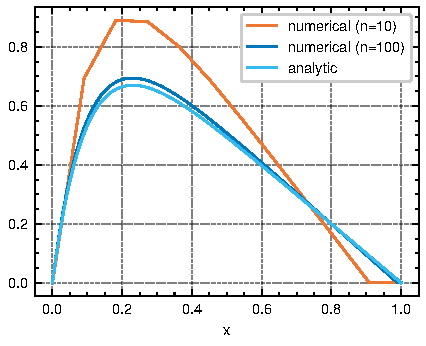
\includegraphics{Figs/problem7.pdf}
    \caption{Numerically computed solutions to the Poisson equation \eqref{eq:Poisson} (with source term given in \eqref{eq:f_x}), using the general algorithm described in section \ref{sec:problem6} for \(n_{\text{steps}}=8\) (green) and \(n_{\text{steps}}=98\) (red). The analytic solution in \eqref{eq:u_x} is shown in blue.}
    \label{fig:v_x}
\end{figure}
In \href{https://github.com/isakrukan/FYS4150/blob/main/Project1/Code/problem7.cpp}{problem7.cpp} the algorithm described in section \ref{sec:problem6}, which we refer to as the ``general algorithm'', is implemented and solves the Poisson equation using \({n_{\text{steps}}\in {10, 100, 1000, 100000}}\), writing to the file \href{https://github.com/isakrukan/FYS4150/blob/main/Project1/Code/problem7.txt}{problem7.txt}. Using the computed values for \(\vec{v}\), Fig. \ref{fig:v_x} is created in \href{https://github.com/isakrukan/FYS4150/blob/main/Project1/Code/problem7.py}{problem7.py}.

Fig. \ref{fig:v_x} shows that the numerically computed solution to the Poisson equation with \(f(x)\) given in \eqref{eq:f_x} quite quickly, seemingly, converges to the analytic solution. Already at \(n_{\text{steps}=100}\) there is no visual difference between the numerical and analytic solution.

\section{Problem 8}
We will now consider the absolute error, which is defined componentwise as
\begin{align}
    (\epsilon_{\text{abs}})_i = \log_{10}|\vec{u}_i-\vec{v}_i|, \label{eq:abs_error}
\end{align}
and the relative error:
\begin{align}
    (\epsilon_{\text{rel}})_i = \log_{10}\big\vert\frac{\vec{u}_i-\vec{v}_i}{\vec{u}_i}\big\vert.   \label{eq:rel_error}
\end{align}
Fig. \ref{fig:abs_error} shows the absolute error \eqref{eq:abs_error} and fig. \ref{fig:rel_error} shows the relative error \eqref{eq:rel_error}, both computed in \href{https://github.com/isakrukan/FYS4150/blob/main/Project1/Code/problem8.py}{problem8.py}, using the values computed in section \ref{sec:problem7}.
\begin{figure}[h!]
    \includegraphics{Figs/problem8_abs_error.pdf}
    \caption{The absolute error between the numerical approximation to the Poisson equation \eqref{eq:Poisson} (with source term given in \eqref{eq:f_x}) using the general algorithm described in section \ref{sec:problem6} for \(n_{\text{steps}}=8\) (green), \(n_{\text{steps}}=98\) (red) and \(n_{\text{steps}}=998\) (blue). }
    \label{fig:abs_error}
\end{figure}



In both figures, the boundary points \(u(0)=u(1)=0\) are excluded. The absolute error in Fig. \ref{fig:abs_error} is mostly constant and decreasing with increasing \(n_{\text{steps}}\), though converges to zero at the \(x=0\) and \(x=1\). This should be expected for any descent numerical approximation, as the analytic solution vanishes at these end points.

The relative error in Fig. \ref{fig:rel_error} is almost perfectly constant for all \(x\in(0,1)\). This supplements the behavior of the absolute error (which is also mostly constant), but also shows that the divergence of the numerical solution from the analytic solution remains constant even when the analytic solution goes to zero at the endpoints.
\begin{figure}[h!]
    \includegraphics{Figs/problem8_rel_error.pdf}
    \caption{The relative error between the numerical approximation to the Poisson equation \eqref{eq:Poisson} (with source term given in \eqref{eq:f_x}) using the general algorithm described in section \ref{sec:problem6} for \(n_{\text{steps}}=8\) (green), \(n_{\text{steps}}=98\) (red) and \(n_{\text{steps}}=998\) (blue). }
    \label{fig:rel_error}
\end{figure}


\begin{table}[h!]
\centering
\begin{tabular}{ |p{3.3cm}|p{3.3cm}|p{1cm}| }
 \hline
 \multicolumn{3}{|c|}{Maximum Absolute and Relative Errors} \\
 \hline
 Absolute error (\(\log_{10}\)) & Relative error (\(\log_{10}\)) & \(n_{\text{steps}}\) \\
 \hline
 \(-1.19\) & \(-1.01\) & \(10^{1}\) \\
 \(-3.24\) & \(-3.07\) & \(10^{2}\) \\
 \(-5.25\) & \(-5.08\) & \(10^{3}\) \\
 \(-7.25\) & \(-7.08\) & \(10^{4}\) \\
 \(-9.04\) & \(-8.84\) & \(10^{5}\) \\
 \(-6.35\) & \(-6.08\) & \(10^{6}\) \\
 \(-6.20\) & \(-5.53\) & \(10^{7}\) \\
 \hline
\end{tabular}
\label{table:errors}
\caption{The maximum absolute and relative errors for \(n_{\text{steps}} = 10^{1}, 10^{2}, ..., 10^{7}\).}
\end{table}
Table \ref{table:errors} shows the maximum absolute and relative errors for \(n_{\text{steps}}= 10^{1}, 10^{2}, ..., 10^{7}\). The table indicates that there is a turning point at \(n_{\text{steps}}\approx 10^{5}\) where the behavior, which prior to \(n_{\text{steps}}\approx 10^{5}\) is that the errors are decreasing for increasing \(n_{\text{steps}}\), starts to increase. 

\section{Problem 9} \label{sec:problem9}
The general algorithm from section \ref{sec:problem6} can be specialized since we know that \(\vec{b}_i=2\) and \(\vec{c}_i = \vec{a}_i=-1\). Concretely, \eqref{eq:tilde_b_ntilde_g} can be written as 
\begin{subequations}    \label{eq:tilde_b_ntilde_g_specialized}
\begin{align}
    \tilde{b}_{i} = 2 - \frac{1}{b_{i-1}}, \quad i=2,..., n,   \label{eq:tilde_b_specialized}\\ 
    \tilde{g}_{i} = h^2f(x_{i+1}) +\frac{g_{i-1}}{b_{i-1}}, \quad i=2,..., n,   \label{eq:tilde_g_specialized}
\end{align}
\end{subequations}
whilst the forward substitution process which led to \eqref{eq:v_i}, can be written as 
\begin{align}
    v_i = \frac{\tilde{g}_{i} + v_{i+1}}{\tilde{b}_{i}}, \quad i = n-1, ..., 1, \label{eq:v_i_specialized}
\end{align}
with \(v_{n} = \tilde{g}_n/\tilde{b}_{n}\). Implementing \eqref{eq:tilde_b_ntilde_g_specialized} requires \({(2+4)*(n-1)}\) FLOPs, while \eqref{eq:v_i_specialized} requires \(3*(n-1)\) (again, counting evaluating \(f\) as a single FLOP), and setting \(v_{n}=\tilde{g}_n/\tilde{b}_n\) requires one. Hence, the total number of FLOPs for the specialized algorithm is \({(2+4)*(n-1) + 3*(n-1) + 1= 9n - 8} \). 


\section{Problem 10}
The special algorithm in section \ref{sec:problem9} requires fewer FLOPs than that of the general algorithm in section \ref{sec:problem6}. Table \ref{table:timings} shows the averaged time duration (over \(100\) runs) of running the general/special algorithm.
\begin{table}[h!]
    \centering
\begin{tabular}{ |p{3.3cm}|p{3.3cm}|p{1cm}| }
 \hline
 \multicolumn{3}{|c|}{Averaged Time Duration of Special/General Algorithm} \\
 \hline
 Special Algorithm [s] & General Algorithm [s] & \(n_{\text{steps}}\)\\
 \hline
 \(1.06 \cdot 10^{-4}\) & \(3.00 \cdot 10^{-5}\) & \(10^{1}\) \\
 \(2.12 \cdot 10^{-4}\) & \(1.18 \cdot 10^{-4}\) & \(10^{2}\) \\
 \(1.64 \cdot 10^{-3}\) & \(1.00 \cdot 10^{-3}\) & \(10^{3}\) \\
 \(2.18 \cdot 10^{-2}\) & \(1.37 \cdot 10^{-2}\) & \(10^{4}\) \\
 \(2.04 \cdot 10^{-1}\) & \(1.26 \cdot 10^{-1}\) & \(10^{5}\) \\
 \(1.94 \cdot 10^{0}\)  & \(1.17 \cdot 10^{0}\)  & \(10^{6}\)
\end{tabular}
\label{table:timings}
\caption{The averaged time duration over \(100\) runs of the special (from section \ref{sec:problem6}) versus the general (from section \ref{sec:problem9}) algorithm. }
\end{table}

\onecolumngrid
% \bibliographystyle{apalike}
\bibliographystyle{unsrt}
\bibliography{ref}


\end{document}